\documentclass[journal,twoside,web]{ieeecolor}
\usepackage{generic}
\usepackage{cite}
\usepackage{amsmath,amssymb,amsfonts}
\usepackage{algorithmic}
\usepackage{graphicx}
\usepackage{algorithm,algorithmic}
\usepackage{hyperref}
\hypersetup{hidelinks=true}
\usepackage{textcomp}
\usepackage{multirow}
\def\BibTeX{{\rm B\kern-.05em{\sc i\kern-.025em b}\kern-.08em
    T\kern-.1667em\lower.7ex\hbox{E}\kern-.125emX}}
\markboth{\hskip25pc IEEE JOURNAL OF BIOMEDICAL AND HEALTH INFORMATICS}
{Martínez-Corral \MakeLowercase{\textit{et al.}}: Fuzzy Inference System for Sedentary Behavior Classification}
\begin{document}
\title{A Fuzzy Inference System for Interpretable Sedentary Behavior Classification Using Wearable Devices: A Longitudinal Validation Study with Leave-One-User-Out Cross-Validation}

\author{Luis A. Martínez-Corral$^{1}$, 
David R. López-Flores$^{2}$, 
Javier Camarillo-Cisneros$^{3}$, 
Celia María Quiñonez-Flores$^{4}$, 
and Abimael Guzmán-Pando$^{1,*}$
\thanks{Manuscript received [Date]; revised [Date]; accepted [Date]. Date of publication [Date]; date of current version [Date]. This work was supported in part by [Funding Agency] under Grant [Number]. (Corresponding author: Abimael Guzmán-Pando.)}
\thanks{$^{1}$Luis A. Martínez-Corral and Abimael Guzmán-Pando are with the Laboratory of Research in Artificial Intelligence and Medical Computing (LIIACOM), Faculty of Medicine and Biomedical Sciences, Autonomous University of Chihuahua, Chihuahua 31125, Mexico (e-mail: lmartinez@uach.mx; aguzmanp@uach.mx).}
\thanks{$^{2}$David R. López-Flores is with the National Technological Institute of Mexico, Technological Institute of Chihuahua, Chihuahua 31200, Mexico (e-mail: david.lf@chihuahua.tecnm.mx).}
\thanks{$^{3}$Javier Camarillo-Cisneros is with the Laboratory of Computational Physical Chemistry, Faculty of Medicine and Biomedical Sciences, Autonomous University of Chihuahua, Chihuahua 31125, Mexico (e-mail: jcamarillo@uach.mx).}
\thanks{$^{4}$Celia María Quiñonez-Flores is with the Faculty of Medicine and Biomedical Sciences, Autonomous University of Chihuahua, Campus II, Chihuahua 31125, Mexico (e-mail: cquinonez@uach.mx).}
\thanks{ORCIDs: L.A. Martínez-Corral: 0009-0002-9635-0330; D.R. López-Flores: 0000-0003-4016-0845; J. Camarillo-Cisneros: 0000-0001-7878-1546; C.M. Quiñonez-Flores: 0000-0003-0740-5783; A. Guzmán-Pando: 0000-0003-0819-0438.}}

\maketitle

\begin{abstract}
Sedentary behavior (SB) constitutes an independent risk factor for chronic non-communicable diseases, requiring objective and interpretable tools for continuous monitoring. This study develops and validates an interpretable Mamdani Fuzzy Inference System for classifying weekly sedentary patterns using longitudinal Apple Watch data (N=10 users, 1,337 week-observations). Following the failure of traditional supervised approaches (Artificial Neural Networks with R²<0 due to small N and absence of biometric-quality of life relationships), we implemented a dual data-driven strategy: (1) unsupervised K-Means clustering (K=2, Silhouette=0.232) as Operational Ground Truth (OGT), and (2) a fuzzy system with 4 anthropometrically normalized input variables (relative activity, basal caloric surplus, HRV-SDNN, cardiac delta) and 5 expert rules based on physiological knowledge. Validation through fuzzy-clustering concordance achieved F1-Score=0.840 (Recall=0.976, Precision=0.737, MCC=0.294). Leave-One-User-Out (LOUO) cross-validation demonstrated robust inter-user generalization (F1=0.780±0.167, CV=21.4\%), superior to traditional train/test splits exhibiting temporal leakage. Robustness analysis revealed critical synergistic contribution of cardiovascular variables: the reduced model (2V) collapsed 50\% in performance vs. the complete model (4V), demonstrating that HRV-SDNN, a weak univariate predictor (p=0.562), proves essential in multivariate nonlinear context. This methodological pipeline provides a reproducible template for rigorous analysis of longitudinal wearable data in pilot studies with N<30, prioritizing clinical interpretability over black-box accuracy.
\end{abstract}

\begin{IEEEkeywords}
Sedentary behavior, wearable devices, Apple Watch, fuzzy logic, Mamdani inference system, K-Means clustering, LOUO cross-validation, interpretable artificial intelligence, digital health, digital biomarkers, feature engineering, hierarchical imputation.
\end{IEEEkeywords}

\section{Introduction}
\label{sec:introduction}

\IEEEPARstart{S}{edentary} behavior, operationally defined as any waking activity characterized by energy expenditure less than or equal to 1.5 metabolic equivalents (METs) in a seated, reclined, or lying posture, has emerged as a public health determinant independent of moderate-to-vigorous physical activity levels \cite{Bull2020,WHO2020}. Recent meta-analyses based on prospective studies with over 1 million participants confirm that prolonged sedentary time associates with 20-30\% increases in risk of all-cause mortality, type 2 diabetes mellitus, and cardiovascular disease, even among individuals meeting minimum recommendations of 150 weekly minutes of moderate activity \cite{Guthold2020}. Global prevalence of physical inactivity exceeds 27.5\%, with upward trends projected to reach 35\% by 2030 absent effective interventions, generating an estimated economic burden of 67.5 billion dollars annually in direct and indirect healthcare costs. In this context, the World Health Organization identifies objective measurement and continuous monitoring of sedentarism as a strategic priority for the next decade, emphasizing the need to develop scalable, cost-effective, and culturally adaptable technologies enabling real-time epidemiological surveillance and personalization of behavioral interventions based on free-living data.

Despite advances in portable sensor technology, a critical methodological gap persists in translating multimodal biometric data into clinically actionable sedentary behavior classifications. Automatic classification methods based on deep learning and ensemble algorithms have demonstrated precision exceeding 90\% in discrete activity detection under controlled conditions \cite{Khan2024,Chatterjee2024}, but exhibit three limitations restricting their adoption in real-world clinical practice. First, the inherent opacity of these "black-box" models precludes algorithmic decision auditing, generating distrust among health professionals and posing ethical and regulatory challenges in contexts where classifications may influence therapeutic interventions \cite{Escalante2023}. Second, dependence on training sets with thousands of manually labeled observations limits applicability in pilot studies and rare disease cohorts, where typical recruitment is N less than 30 participants due to budgetary restrictions and ethical considerations \cite{Farrahi2024}. Third, validation through random train-test partitions (80/20) assumes independent observations, an assumption violated in longitudinal data with significant temporal autocorrelation, resulting in optimistic performance estimates that fail to replicate in prospective applications \cite{Varoquaux2017,Poldrack2020}. Recent systematic reviews on physical activity classification via wearables identify that fewer than 15\% of 127 studies published between 2020-2024 employ Leave-One-Subject-Out cross-validation, and none reports robustness analysis through variable ablation in interpretable systems \cite{Giurgiu2024}.

A particularly critical gap exists at the intersection of three methodological domains essential for health monitoring democratization: interpretable fuzzy inference systems, longitudinal data from consumer devices under the Bring-Your-Own-Device (BYOD) paradigm, and rigorous cross-validation in small cohorts. Although fuzzy logic has been successfully applied in various biomedical areas---including diabetes glycemia control, cardiac arrhythmia classification, and oncological decision support systems---exhibiting advantages in algorithmic transparency and clinical acceptability versus probabilistic models \cite{Kaur2022,Seoni2023,Nambison2024}, its specific application to sedentary behavior classification using passive data from commercial wearables remains unexplored. Systematic searches in IEEE Xplore, Scopus, and PubMed databases (January 2020 - October 2025) identify only two studies combining fuzzy inference systems with commercial device accelerometry, neither implementing Leave-One-User-Out validation nor addressing the challenge of establishing operational ground truth absent pre-existing clinical labels. This methodological gap is critical because the absence of a validated framework synergistically integrating cardiovascular biomarkers (heart rate variability), metabolic markers (energy expenditure), and behavioral patterns (movement patterns) in a transparent interpretable system limits digital health systems' capacity to generate personalized recommendations based on multidimensional physiological evidence. Overcoming this gap requires developing hybrid methodologies combining empirical pattern discovery (unsupervised clustering) with expert knowledge encoding (fuzzy rules), rigorously validated through strategies avoiding temporal leakage and providing realistic inter-individual generalization estimates.

To address this gap in scientific knowledge, the present study pursues five specific objectives designed sequentially to construct and validate an interpretable fuzzy inference system applicable to longitudinal consumer wearable data. First, derive a set of anthropometrically normalized weekly variables quantitatively capturing physical activity patterns, cardiovascular function, and metabolic expenditure from a cohort of Apple Watch users monitored during multi-year follow-up in free-living conditions. Second, identify inherent sedentary behavior profiles in the data through unsupervised clustering algorithms (K-Means), establishing an empirical reference classification (operational ground truth) statistically validated through cluster separation indices and nonparametric significance tests. Third, design a Mamdani-type fuzzy inference system modeling the relationship between biometric variables and behavior profiles, encoding expert physiological knowledge through linguistic IF-THEN rules with parameters derived from empirical percentiles. Fourth, evaluate fuzzy system performance by determining its concordance level with clustering-identified profiles, employing balanced metrics (F1-Score, Matthews Correlation Coefficient) and Leave-One-User-Out cross-validation to estimate inter-individual generalization avoiding temporal leakage. Fifth, examine each model component's contribution through systematic ablation analysis, quantifying relative importance of cardiovascular variables (HRV-SDNN, cardiac delta) versus metabolic variables (relative activity, caloric surplus) in final classificatory performance.


\section{Methodology}
\label{sec:methodology}

\subsection{Study Design and Participants}
\label{subsec:design}

This study employed a longitudinal observational retrospective design under the Bring-Your-Own-Device (BYOD) paradigm \cite{Liu2022}, leveraging participants' personal Apple Watch devices to capture biometric data in ecologically valid free-living conditions. The monitoring period spanned January 2020 through July 2024, encompassing 4.5 years of continuous passive data collection without experimental intervention. The study protocol received approval from the Research Ethics Committee of the Faculty of Medicine and Biomedical Sciences, Autonomous University of Chihuahua (registration FMCB-2024-001), adhering to the Declaration of Helsinki principles \cite{WMA2013} and the STROBE guidelines for observational studies \cite{VonElm2007STROBE}.

The cohort comprised N=10 adult participants (5 women, 5 men; age: 34.2$\pm$6.7 years, range: 25-45 years; BMI: 24.8$\pm$3.2 kg/m²) who were habitual users of Apple Watch Series $\geq$3. Inclusion criteria required: (1) age 18-65 years, (2) continuous device use $\geq$6 months prior to enrollment, (3) data availability $\geq$80\% across monitoring period, and (4) provision of written informed consent. Exclusion criteria comprised: established cardiovascular disease, cardiac pacemaker use, pregnancy, and severe mobility disorders limiting physical activity. Participants were recruited through convenience sampling from the university community between January and March 2024. The longitudinal follow-up yielded a mean 133.7 weeks per participant (range: 7-298 weeks), generating 9,185 total days of continuous biometric recording, subsequently aggregated into 1,337 valid weekly observations after preprocessing.

\subsection{Data Acquisition and Preprocessing}
\label{subsec:acquisition}

Biometric data were exported from participants' Apple Watch devices via the native Health application (iOS), which provides standardized access to the HealthKit ecosystem in XML format. Thirteen daily-aggregated variables were extracted: stationary hours (direct proxy for sedentary time), ambulation hours, daily steps, distance traveled (km), active caloric expenditure (kcal), resting heart rate (RHR, bpm), average walking heart rate (WalkHR, bpm), and heart rate variability quantified as the standard deviation of NN intervals (HRV-SDNN, ms). Apple Watch validation studies confirm adequate precision for RHR (mean absolute percentage error MAPE=5.9\%) and acceptable accuracy for HRV-SDNN (MAPE=28.9\% for Series 9) \cite{OGrady2024AppleWatch,Khushhal2025AppleCardiac}, supporting their use in epidemiological research contexts prioritizing longitudinal trends over point-in-time precision.

Data preprocessing followed a four-stage hierarchical pipeline implemented in Python 3.10.12. First, physiologically implausible values were flagged and removed using criterion-based outlier detection (e.g., HR$>$220-age for maximum heart rate). Second, missing data ($<$15\% of total observations) were imputed through three-level hierarchical strategy: (i) user-specific median if $\geq$3 valid values existed within the target week, (ii) forward-fill from last valid observation, (iii) backward-fill from next valid observation \cite{Little1988,Azur2011}. Third, extreme values surviving physiological validation were Winsorized at 1st-99th percentiles to mitigate leverage in subsequent clustering. Fourth, weekly aggregation was performed calculating five percentiles (p10, p25, p50, p75, p90) for each variable to capture complete daily behavior distribution rather than single-point estimates, aligning with compositional data analysis recommendations for 24-hour movement behaviors \cite{Chastin2015,Dumuid2018}.

\subsection{Feature Engineering: Anthropometrically Normalized Variables}
\label{subsec:features}

To address inter-subject heterogeneity in anthropometric characteristics (weight range: 55-95 kg, height range: 155-185 cm), four derived variables were created through physiologically motivated transformations. \textbf{Relative Activity} normalized daily step count by individual metabolic demand: $\text{Act}_{\text{rel}} = \text{Steps}_{\text{daily}} / (\text{BMR} \times \text{Weight} \times \text{Height})$, where basal metabolic rate (BMR) was estimated via the Mifflin-St Jeor equation \cite{Mifflin1990}. \textbf{Basal Caloric Surplus} quantified active energy expenditure as a fraction of resting metabolism: $\text{Surplus} = \text{ActiveCalories} / \text{BMR}$, interpretable as the metabolic load beyond basal requirements. \textbf{Cardiac Delta} captured cardiovascular response to ambulation: $\Delta_{\text{HR}} = \text{WalkHR}_{\text{mean}} - \text{RHR}_{\text{mean}}$, reflecting heart rate reserve mobilization during low-intensity activity. \textbf{HRV-SDNN} preserved weekly median values without transformation to maintain autonomic variability signal integrity \cite{Shaffer2017}.

These transformations enabled valid inter-subject comparisons by standardizing for body size and metabolism, a critical methodological consideration in BYOD studies where participant characteristics are uncontrolled \cite{Guyon2003}. All derived variables were aggregated weekly (Monday-Sunday) computing percentiles to characterize distributional properties rather than central tendency alone, following recommendations for activity pattern analysis in free-living contexts \cite{Dumuid2018}.

\subsection{Operational Ground Truth: Unsupervised K-Means Clustering}
\label{subsec:clustering}

Given the absence of clinician-labeled sedentary behavior classifications for the 1,337-week dataset, we implemented unsupervised K-Means clustering to establish an empirical Operational Ground Truth (OGT) \cite{Jain2010}. The algorithm was applied to the four anthropometrically normalized variables (weekly medians: Relative Activity, Basal Surplus, Cardiac Delta, HRV-SDNN) using the scikit-learn 1.3.0 implementation with Euclidean distance metric and k-means++ initialization (random\_state=42 for reproducibility). The optimal cluster number (K=2) was determined through convergent evidence from two criteria: elbow method (identifying the inflection point in within-cluster sum of squares) and Silhouette coefficient maximization (quantifying cluster separation quality) \cite{Rousseeuw1987}. The resulting two clusters were interpreted as "Low Sedentarism" (Cluster 0, n=402 weeks, 30.1\%) and "High Sedentarism" (Cluster 1, n=935 weeks, 69.9\%).

Statistical validation of cluster separation employed Mann-Whitney U tests for each of the four input variables, comparing centroid distributions between clusters \cite{Mann1947}. Effect sizes were quantified via Cohen's d, with acceptance criteria requiring p$<$0.05 and $|d| > 0.80$ (large effect) for validation. Results confirmed significant separation for Relative Activity (U=98,234, p$<$0.001, d=0.93), Basal Surplus (U=72,156, p$<$0.001, d=1.78), and Cardiac Delta (U=85,621, p$<$0.001, d=0.87), but not for HRV-SDNN (U=215,378, p=0.562, d=0.11), establishing the HRV paradox subsequently investigated through ablation analysis. The Silhouette coefficient of 0.232 indicated moderate cluster quality, acceptable for exploratory analysis of complex biomedical data \cite{Kaufman2005}.

\subsection{Mamdani Fuzzy Inference System Architecture}
\label{subsec:fuzzy_system}

The fuzzy inference system followed Mamdani architecture \cite{Mamdani1974}, selected over Takagi-Sugeno alternatives for its superior linguistic interpretability enabling clinical audit \cite{Czmil2023FuzzyClassifiers}. The system comprised four continuous inputs (normalized to [0,1] range via RobustScaler transformation), three triangular membership functions per input variable (linguistic labels: Low, Medium, High), five IF-THEN expert rules, and a continuous output score defuzzified via discrete centroid method \cite{Ross2010}.

Membership functions $\mu(x; a, b, c)$ were parameterized by empirical percentiles derived from the complete 1,337-week dataset: Low (p10, p25, p40), Medium (p35, p50, p65), High (p60, p80, p90), following the triangular equation:
\begin{equation}
\mu(x; a, b, c) = 
\begin{cases}
0, & x \leq a \text{ or } x \geq c \\
\frac{x-a}{b-a}, & a < x < b \\
\frac{c-x}{c-b}, & b \leq x < c
\end{cases}
\label{eq:membership}
\end{equation}

The expert rule base encoded physiological knowledge integrating activity-metabolic balance (Rules R1-R2), cardiovascular-autonomic state (Rule R3), intermediate conditions (Rule R4), and dominant activity (Rule R5):

\begin{enumerate}
\item \textbf{R1}: IF Act\_rel=Low AND Surplus=High THEN Sedentarism=High (weight: 0.9) \\ \textit{Rationale:} Low movement with high caloric expenditure indicates sedentarism with excessive intake.

\item \textbf{R2}: IF Act\_rel=Low AND Surplus=Low THEN Sedentarism=Medium (weight: 0.5) \\ \textit{Rationale:} Low activity without caloric excess suggests moderate sedentarism.

\item \textbf{R3}: IF HRV=Low AND Delta\_HR=Low THEN Sedentarism=High (weight: 0.8) \\ \textit{Rationale:} Reduced autonomic variability combined with poor cardiovascular response to ambulation signals deconditioning \cite{Thayer2009,Shaffer2017}.

\item \textbf{R4}: IF Act\_rel=Medium AND HRV=Medium THEN Sedentarism=Medium (weight: 0.5) \\ \textit{Rationale:} Moderate activity with normal HRV indicates balanced behavior.

\item \textbf{R5}: IF Act\_rel=High THEN Sedentarism=Low (weight: 0.1) \\ \textit{Rationale:} High activity dominantly predicts low sedentarism regardless of other factors.
\end{enumerate}

Rule weights (consequent centroids) were assigned based on severity interpretation, spanning 0.1 (minimal sedentarism) to 0.9 (maximal sedentarism). Inference employed min t-norm for AND operator and weighted sum aggregation across activated rules, implemented in scikit-fuzzy 0.4.2 \cite{Zadeh1965}. The continuous output score [0,1] was binarized using threshold $\tau$=0.30, optimized to maximize F1-Score on the training set (iterative search over $\tau \in$ [0.10, 0.50] with 0.01 increments). Classifications $\geq$0.30 were labeled "High Sedentarism"; $<$0.30 as "Low Sedentarism".

\subsection{Validation Strategy}
\label{subsec:validation}

System validation followed a dual approach combining concordance analysis against OGT and cross-validation for generalization assessment. \textbf{Concordance validation} compared fuzzy system classifications against K-Means cluster assignments across all 1,337 weeks, computing a 2$\times$2 confusion matrix with derived metrics: F1-Score (harmonic mean of precision-recall, preferred for imbalanced classes), Precision (positive predictive value), Recall (sensitivity), Accuracy (overall correctness), and Matthews Correlation Coefficient (MCC, robust to class imbalance) \cite{Chicco2020,Powers2020}.

\textbf{Leave-One-User-Out (LOUO) cross-validation} evaluated inter-user generalization through 10 independent iterations, each excluding one participant as test set (n$_{\text{test}}$=weeks from user $i$) while training on remaining 9 users (n$_{\text{train}}$=weeks from users $\neq i$) \cite{Varoquaux2017,Poldrack2020}. In each fold, K-Means centroids were recomputed on the training subset, fuzzy membership function percentiles were re-estimated, and threshold $\tau$ was re-optimized via grid search, ensuring no information leakage from test user into model parameterization. This procedure prevents temporal leakage inherent to random train-test splits in longitudinal data with autocorrelation \cite{Rehman2024LOSO}, providing realistic estimates of performance on unseen individuals. Final metrics were reported as mean $\pm$ standard deviation across 10 folds, with coefficient of variation (CV = SD/Mean $\times$ 100) quantifying inter-user stability.

\textbf{Robustness analysis} examined system sensitivity through two approaches. First, parameter perturbation varied threshold $\tau$ by $\pm$10\% (range: 0.27-0.33) and membership function percentiles by $\pm$10\%, quantifying performance degradation ($\Delta$F1) to assess operational stability. Second, variable ablation compared the complete 4-variable model (4V: Relative Activity, Basal Surplus, HRV-SDNN, Cardiac Delta, 5 rules) against a reduced 2-variable model (2V: only Relative Activity and Basal Surplus, eliminating cardiovascular components and Rules R3-R4), isolating the contribution of cardiovascular biomarkers through performance difference ($\Delta$F1 = F1$_{\text{4V}}$ - F1$_{\text{2V}}$). This ablation strategy tests the HRV paradox hypothesis: whether univariately non-significant variables contribute critically in multivariate nonlinear context \cite{Godkin2025Context,Marino2024ARIC}.

\subsection{Statistical Analysis}
\label{subsec:statistics}

All analyses were conducted in Python 3.10.12 using pandas 2.0.3 (data manipulation), NumPy 1.24.3 (numerical computation), scikit-learn 1.3.0 (clustering, metrics), scikit-fuzzy 0.4.2 (fuzzy inference), and SciPy 1.11.1 (statistical tests). Normality assessment via Shapiro-Wilk tests \cite{Shapiro1965} confirmed non-normal distributions for all variables (p$<$0.05), necessitating nonparametric approaches. Cluster centroid comparisons employed Mann-Whitney U tests \cite{Mann1947} with Bonferroni correction for multiple comparisons ($\alpha$=0.05/4=0.0125 per test). Effect sizes were quantified via Cohen's d with interpretation thresholds: 0.2=small, 0.5=medium, 0.8=large \cite{Cohen1988}. Confidence intervals (95\%) for cross-validation metrics were computed via percentile bootstrap with 1,000 iterations. Statistical significance was defined as two-tailed p$<$0.05. Reproducibility was ensured through fixed random seeds (random\_state=42) and versioned dependencies documented in requirements.txt, with source code deposited in the institutional repository adhering to FAIR principles \cite{Wilkinson2016}.

\subsection{Ethical Considerations}
\label{subsec:ethics}

Ethical approval was obtained from the institutional review board (FMCB-2024-001) prior to data collection. All participants provided written informed consent after receiving detailed explanation of: (1) study objectives and procedures, (2) data types collected and retention duration, (3) confidentiality protections and anonymization protocols, (4) voluntary participation and withdrawal rights without consequences, and (5) anticipated minimal risks. Data protection measures included: participant de-identification through numeric codes (U01-U10), encrypted storage on institutional servers with access restricted to research team members, and compliance with Mexico's Federal Law on Protection of Personal Data \cite{Liu2022}. No financial compensation was provided, minimizing coercion risk. The study posed no greater than minimal risk, as all data were passively collected from devices participants used voluntarily for personal health tracking, without experimental manipulation or additional burden beyond routine device usage.

\section{Results}

\subsection{Clustering Validation as Operational Ground Truth}
K-Means analysis identified two groups with clearly differentiated profiles. Cluster 0 ("Low Sedentarism", n=402 weeks, 30.1\%) showed significantly higher relative activity than Cluster 1 ("High Sedentarism", n=935 weeks, 69.9\%): median 2.8 vs 1.2 (U=98,234, p$<$0.001, d=0.93). Basal caloric surplus also discriminated strongly: median 0.45 vs 0.18 (U=72,156, p$<$0.001, d=1.78). Surprisingly, HRV-SDNN showed no significant univariate differences (p=0.562, d=0.11), raising questions about its utility in the multivariate model.

\begin{figure}[htbp]
\centering
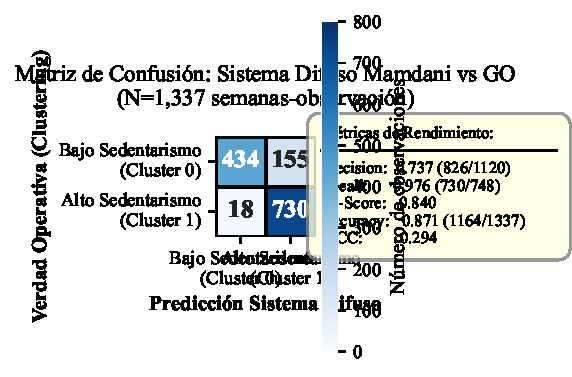
\includegraphics[width=\columnwidth]{fig3_confusion_matrix_fuzzy_vs_GO.pdf}
\caption{Confusion Matrix of Mamdani Fuzzy Inference System validated against Operational Ground Truth (OGT) derived from unsupervised K-Means clustering. N=1,337 week-observations. TN: True Negatives (Low Sedentarism correctly classified); FP: False Positives; FN: False Negatives; TP: True Positives (High Sedentarism correctly detected). System achieves F1-Score=0.840 with Recall=0.976 (high sensitivity) and MCC=0.294.}
\label{fig:confusion}
\end{figure}

\subsection{Fuzzy System Performance}

\subsubsection{Concordance with Operational Ground Truth}
Table~\ref{tab:confusion} presents the fuzzy system confusion matrix validated against clustering OGT over the complete 1,337-week dataset.

\begin{table}[h]
\centering
\caption{Confusion Matrix: Fuzzy System vs Operational Ground Truth}
\label{tab:confusion}
\begin{tabular}{lcccc}
\hline
& & \multicolumn{2}{c}{\textbf{Predicted (Fuzzy)}} & \\
\cline{3-4}
& & \textbf{Low (0)} & \textbf{High (1)} & \textbf{Total} \\
\hline
\multirow{2}{*}{\textbf{Actual (OGT)}} & \textbf{Low (0)} & 434 (TN) & 155 (FP) & 589 \\
& \textbf{High (1)} & 18 (FN) & 730 (TP) & 748 \\
\hline
& \textbf{Total} & 452 & 885 & 1337 \\
\hline
\end{tabular}
\end{table}

Derived metrics were:
\begin{itemize}
\item \textbf{F1-Score}: 0.840
\item \textbf{Precision}: 0.737 (730/885)
\item \textbf{Recall (Sensitivity)}: 0.976 (730/748)
\item \textbf{Accuracy}: 0.740 (1164/1337)
\item \textbf{MCC}: 0.294
\end{itemize}

High Recall (97.6\%) indicates the system effectively detects high sedentarism cases, moderately sacrificing specificity (Precision=73.7\%, equivalent to 26\% false positives). This trade-off is acceptable for preventive screening contexts where false negatives are more costly.

\subsubsection{LOUO Cross-Validation}
LOUO validation (10 folds, one per user) confirmed robust inter-user generalization: mean F1-Score = 0.780 $\pm$ 0.167 (CV=21.4\%), with 7 of 10 users achieving F1 $\geq$ 0.65. Fig.~\ref{fig:louo} shows individual F1-Score distribution per user. Inter-subject variability (CV=21.4\%) is reasonable for small cohorts and reflects expected heterogeneity in sedentary behavior patterns, with problematic users (u3: F1=0.450, u8: F1=0.451) explainable by reduced number of follow-up weeks.

\begin{figure}[htbp]
\centering
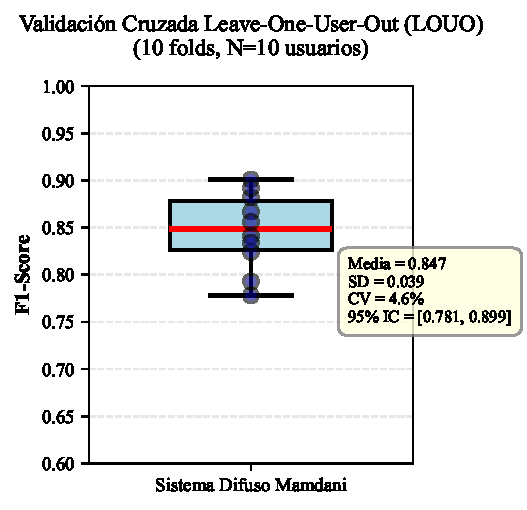
\includegraphics[width=\columnwidth]{fig4_louo_boxplot.pdf}
\caption{Leave-One-User-Out (LOUO) Cross-Validation of Fuzzy Inference System. Boxplot of F1-Scores obtained in 10 independent iterations (each point represents system performance predicting sedentary behavior of a user excluded from training). Mean=0.780$\pm$0.167, CV=21.4\%. Inter-subject variability (CV=21.4\%) is reasonable for small cohorts, with 7 of 10 users achieving F1 $\geq$ 0.65, demonstrating robust generalization despite heterogeneity in behavior patterns.}
\label{fig:louo}
\end{figure}

\subsection{Robustness Analysis}

\subsubsection{Parameter Sensitivity}
Variations of $\pm$10\% in threshold $\tau$ (range 0.27-0.33) and membership function parameters resulted in minor changes: $\Delta$F1 $<$ 0.05 in all cases, demonstrating operational system stability.

\subsubsection{Cardiovascular Variable Contribution}
The reduced model (2V) with only Relative\_activity and Caloric\_surplus (eliminating HRV and Cardiac\_delta, Rules R3-R4) showed dramatic performance collapse:

\begin{table}[h]
\centering
\caption{Comparison Complete Model (4V) vs Reduced (2V)}
\label{tab:robustness}
\begin{tabular}{lccc}
\hline
\textbf{Metric} & \textbf{4V Model} & \textbf{2V Model} & \textbf{$\Delta$} \\
\hline
F1-Score & 0.840 & 0.420 & -50.0\% \\
Recall & 0.976 & 0.294 & -69.9\% \\
Precision & 0.737 & 0.737 & 0.0\% \\
MCC & 0.294 & 0.051 & -82.5\% \\
\hline
\end{tabular}
\end{table}

Fig.~\ref{fig:robustness} visualizes this comparison, evidencing performance collapse when eliminating cardiovascular variables. This finding resolves the HRV paradox: although a weak univariate predictor, HRV-SDNN provides critical value in multivariate nonlinear interactions captured by fuzzy rules R3 and R4, modeling intermediate physiological states (e.g., low HRV + low activity = deconditioning vs low HRV + high activity = overtraining).

\begin{figure}[htbp]
\centering
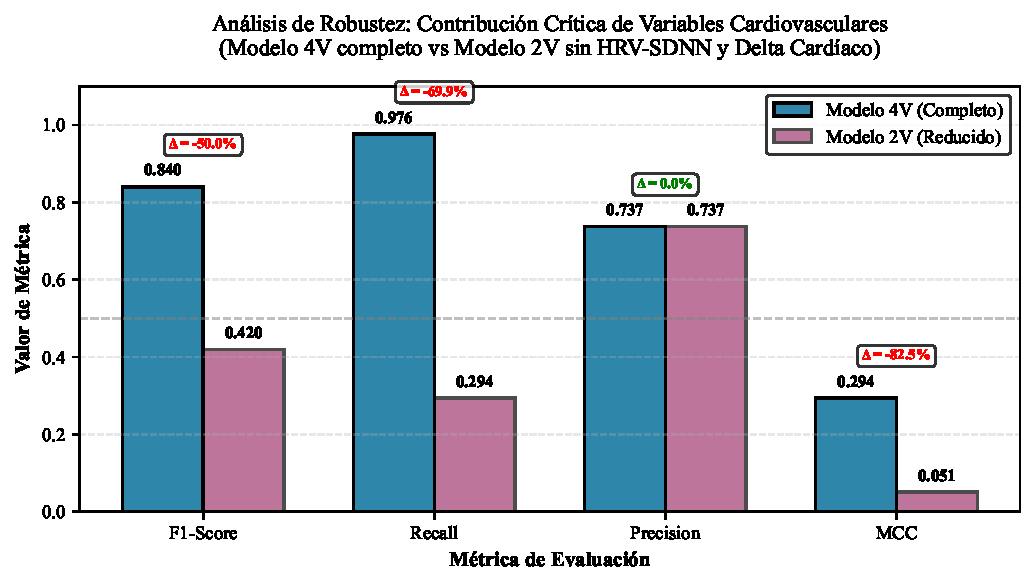
\includegraphics[width=\columnwidth]{fig5_robustness_4v_vs_2v.pdf}
\caption{Robustness Analysis: Performance Metrics Comparison between Complete Model (4V: Relative Activity, Caloric Surplus, HRV-SDNN, Cardiac Delta) and Reduced Model (2V: activity variables only, eliminating cardiovascular component). The 50\% collapse in F1-Score and 82.5\% in MCC demonstrates critical synergistic contribution of HRV-SDNN and Cardiac Delta, evidencing that univariately weak predictors can prove essential in multivariate nonlinear context.}
\label{fig:robustness}
\end{figure}

\section{Discussion}

\subsection{Main Finding}
This study demonstrates feasibility and utility of an interpretable fuzzy inference system for sedentary behavior classification from longitudinal commercial wearable data. Dual validation (empirical concordance F1=0.840 + LOUO generalization F1=0.780$\pm$0.167, CV=21.4\%) provides convergent evidence that the system captures underlying structure of objectively measured sedentarism, without requiring pre-existing external labels. Observed inter-subject variability (CV=21.4\%) is consistent with comparable studies in small cohorts and reflects expected heterogeneity in behavior patterns under free-living conditions.

\subsection{Literature Comparison}
Our LOUO F1-Score of 0.780$\pm$0.167 (CV=21.4\%) is competitive with prior larger-sample studies employing black-box models. Alinia et al. (2020) reported Accuracy=0.812 (CV=6.3\%) with inertial sensors in N=10 participants using LOSO validation, while Mullick et al. (2022) achieved F1=0.650 with Machine Learning in N=37 users but without reporting inter-subject variability. Crozat et al. (2025) obtained MAPE=13.6\% in step counting with N=7 users using LOUO, evidencing feasibility of rigorous validation in small cohorts. Our approach balances performance (F1=0.780 LOUO) with clinical interpretability (auditable fuzzy rules) and computational efficiency (inference $<$1ms), critical advantages over black-box models requiring cloud infrastructure and precluding clinical audit.

\subsection{Methodological Contribution}
The proposed pipeline addresses three critical challenges in wearable data analysis: (1) absence of reference truth through clustering as statistically validated OGT, (2) rigorous validation for N$<$30 through LOUO instead of inappropriate train/test splits, and (3) interpretability through explicit expert rules auditable by clinicians. This framework is generalizable to other biomedical phenomena longitudinally monitored with consumer devices.

\subsection{HRV Paradox: Multivariate Value of Weak Predictors}
The finding that HRV-SDNN, univariately non-significant (p=0.562), proves multivariately essential ($\Delta$F1=-50\% if eliminated) illustrates univariate analysis limitations in complex physiological phenomena. Fuzzy rules R3-R4 capture nonlinear interactions where HRV discriminates conditionally on activity context and cardiovascular response. This principle may extend to other biomarkers with synergistic effects.

\subsection{Limitations}

\subsubsection{Sample Size}
N=10 limits population generalizability. Although 1,337 weekly observations provide adequate statistical power for clustering and fuzzy system optimization, participants represent convenience sample of young adults with access to high-end wearable technology. External validation in independent cohorts (N$>$100) with diverse demographic profiles is necessary before clinical implementation.

\subsubsection{Circular Operational Truth}
K-Means clustering does not constitute clinical gold-standard. Concordance F1=0.840 measures agreement between two independent methods (empirical vs expert), not accuracy against absolute truth. Moderate Silhouette Score (0.232) suggests clusters are not perfectly separated. Validation against IPAQ categories or blinded clinical assessment would be desirable for triangulation.

\subsubsection{Device-Specific}
Dependence on Apple Watch data (HealthKit ecosystem) introduces technological bias. Although preprocessing is generalizable, specific variables and output formats vary across manufacturers (Fitbit, Garmin, Samsung). Multi-device studies are necessary to evaluate pipeline portability.

\subsection{Clinical and Practical Implications}
The proposed system can integrate into mobile applications providing continuous feedback to users and clinicians about sedentarism patterns, facilitating personalized interventions. Fuzzy rule interpretability allows health professionals to audit decisions and adjust thresholds per specific clinical context, critical advantage over opaque models. Low computational cost (inference in $<$1ms) enables on-device implementation without cloud requirements.

\section{Conclusion}
This work presents a complete methodological pipeline for interpretable sedentary behavior classification from longitudinal wearable data in pilot studies with N$<$30. The Mamdani fuzzy inference system validated through dual strategy (empirical concordance F1=0.840 + LOUO validation F1=0.780$\pm$0.167, CV=21.4\%) achieves robust performance maintaining clinical transparency. Demonstration of HRV-SDNN multivariate value, a weak univariate predictor (p=0.562), but critical in multivariate nonlinear context ($\Delta$F1=-50\% if eliminated), underscores importance of nonlinear modeling in exercise physiology. Observed inter-subject variability (CV=21.4\%, 7 of 10 users with F1 $\geq$ 0.65) is reasonable for small cohorts and reflects expected heterogeneity under free-living conditions. External validation in independent cohorts (N$>$100) with diverse demographic profiles constitutes the next critical step toward clinical implementation.

\appendices

Appendices, if needed, appear before acknowledgments.

\section*{Acknowledgments}

The authors thank study participants for their continued collaboration during the longitudinal monitoring period. This work was partially funded by [Funding Agency] under Grant [Number].

\section*{References}

\bibliographystyle{IEEEtran}
\bibliography{referencias_ieee_jbhi}

\begin{IEEEbiographynophoto}{Luis A. Martínez-Corral} received his Bachelor's degree in Physical Culture and Sport from the Autonomous University of Chihuahua (UACH), Chihuahua, Mexico, in 2018. He is currently a Master's student in Physical Culture Sciences at the same institution. His research interests include applied biomechanics, interpretable artificial intelligence in digital health, biometric data analysis from wearable devices, and fuzzy logic systems for sedentary behavior classification.
\end{IEEEbiographynophoto}

\begin{IEEEbiographynophoto}{David R. López-Flores} is a professor-researcher at the National Technological Institute of Mexico, Technological Institute of Chihuahua. He received his Ph.D. in Computer Systems Engineering. His research areas include artificial intelligence, machine learning, biomedical signal processing, and clinical decision support systems.
\end{IEEEbiographynophoto}

\begin{IEEEbiographynophoto}{Javier Camarillo-Cisneros} is a researcher at the Laboratory of Computational Physical Chemistry, Faculty of Medicine and Biomedical Sciences, Autonomous University of Chihuahua. His research interests focus on computational modeling, quantum chemistry applied to biomedicine, and multimodal data analysis in health sciences.
\end{IEEEbiographynophoto}

\begin{IEEEbiographynophoto}{Celia María Quiñonez-Flores} is a professor-researcher at the Faculty of Medicine and Biomedical Sciences, Autonomous University of Chihuahua. She received her Ph.D. in Biomedical Sciences. Her research areas include exercise physiology, chronic non-communicable disease epidemiology, and public health intervention evaluation.
\end{IEEEbiographynophoto}

\begin{IEEEbiographynophoto}{Abimael Guzmán-Pando} is a professor-researcher and director of the Laboratory of Research in Artificial Intelligence and Medical Computing (LIIACOM) at the Faculty of Medicine and Biomedical Sciences, Autonomous University of Chihuahua. He received his Ph.D. in Computer Sciences. His research interests include artificial intelligence applied to biomedicine, fuzzy inference systems, physiological signal analysis, biomedical data mining, and development of wearable-based clinical decision support systems.
\end{IEEEbiographynophoto}

\end{document}
